% !TEX root = ../report.tex

\chapter{System Testing}\label{systest}
System testing took place following integration testing and
the full construction of the robot. The aim of system testing is to ensure that
each of the component parts work as expected when integrated together, and to
test and evaluate the system as a whole. A modular
maze testing environment was used throughout integration and
system testing to allow as many different maze configurations
as possible to be tested. Throughout integration the modular maze was used as a
``SLAM playground'', where various sized boxes or simple two area configurations
were used to test the robot's capabilities in these environments and assess the
SLAM maps built when using these configurations.
\section{Modular Maze}\label{test/maze}
The modular maze environment was designed with the aim of being able to system
test on as many maze configurations as possible. By creating a modular
environment, the maze was also reusable in future iterations of the project, or
similar projects which required a secure area to test small autonomous vehicles.
\subsection{Design}\label{test/maze/design}
With these broad specifications in mind, a list of requirements for the maze
environment was created (see Table~\ref{maze_reqs}).

\begin{table}[!ht]\centering
\caption{Modular maze requirements
\label{maze_reqs}}
    \begin{tabular}{ccc}
        \toprule
        \thead{Requirement} & \thead{Priority}\\
        \midrule
        Be easily modifiable & High\\
        Have enough cells to allow varied mazes & High\\
        Have minimum cell width $>$ diameter of the robot & High\\
        Be accompanied by sufficient ``pegs'' and ``walls'' to build complex 		mazes & High\\
        Wall material be non-translucent and non-reflective & Medium\\
        Base material be non-reflective & Medium\\
        Maze be easily transportable & Medium\\
        Maze base be modular & Low\\
        \bottomrule
    \end{tabular}
\end{table}

These requirements were then used to create a number of approximate ideas which
were presented to the mechanical workshop. The maze base would be
\SI{1280 x 1690 x 18}{\mm}, giving 7 columns by 9 rows of
peg holes each \SI{12}{\mm} in diameter and \SI{210}{\mm} from centre to
centre. The holes drilled into the maze base would be \SI{15}{\mm} in depth
leaving a \SI{3}{\mm} section of the base board un-drilled within the hole for the peg to rest on. The pegs would then be
\SI{165}{\mm} in height, a protrusion of \SI{150}{\mm} from the top of the base board, with a cross slit cut from the top to
roughly \SI{75}{\mm} down the peg
(half the visible portion). These slits would be approximately \SI{3}{\mm} wide to allow the walls to be slotted in. For
this to be accomplished, the walls would be winged---\SI{208}{\mm} in length at the top and \SI{196}{\mm} in length
\SI{75}{\mm} from the top. This gives \SI{6}{\mm} spaces at either side to allow for the diameter of the peg and means the walls
can be slotted between two pegs with ease.

The materials required were researched to obtain the measurements
above, such as \SI{12}{\mm} being a standard size for wood dowel and \SI{3}{\mm}
and \SI{18}{\mm} respectively being depths of MDF which could be used for the
walls and base boards. These requirements, descriptions and accompanying
drawings were delivered to the mechanical workshop for construction to begin.

\subsection{Implementation}\label{test/maze/impl}
The mechanical workshop required a number of changes to the original design in
order for the maze to be created.

Foremost, the largest single item of solid wood which could be obtained from
suppliers was smaller than the requested measurements of \SI{1280 x 1690 x 18}
{\mm}. Two resolutions were proposed by the mechanical workshop: reduce
the width of each cell, or remove a column and row of holes from the maze. Following
team consultation, it was decided that reducing the size of each cell would
result in more flexibility in the end product, as 3 columns of two cell wide paths could still
be created. It is also worth noting that the reduced cell width of \SI{195}{\mm}
still met the requirement of the cell width being larger than the diameter of
the robot.

Secondly, the materials used for the walls and pegs would not be wood as this
would involve many man hours to create the slits in the dowel and
manually cut the walls to size. In order to streamline the process, it was
suggested by the mechanical workshop, that the walls be made of acrylic, allowing
them to be laser cut, and the pegs be 3D printed, allowing mass printing
once a design had been finalised. It was agreed amongst the group that this was a good idea and
in order for the pegs to be 3D printed they had to be made using CAD modelling
software. None of the group had experience using this software, hence
a steep learning curve was involved in carrying out this task.

A peg matching the original specifications was modelled, however upon delivery
to the mechanical workshop, the group were informed that this design had to be
changed to allow the walls to be cut as rectangles only---with no wings. A new
peg design was created which had slits at each \SI{90}{\degree} interval,
running the length of the peg and leaving a central column intact. This allowed the wall to be dropped in without
the need for wings. This peg design was also modelled.

Upon returning to the mechanical workshop the group were once again informed
that the peg design had to be altered. The base board had been drilled through
and so the pegs now required a smaller peg on the bottom and a rim to ensure
that they did not fall through the base board. The agreed design was the same as
previously with the peg now having a diameter of \SI{15}{\mm} with the small peg
at the bottom having the original \SI{12}{\mm} diameter and \SI{15}{\mm} in
height. The design was agreed and the peg was modelled.

Midway through modelling the group were called by the mechanical workshop and
informed that the acrylic which had been ordered was slightly wider than the
originally thought \SI{3}{\mm} and so the slits would have to be widened to
\SI{4}{\mm} to allow for this. The model was altered to account for this change and delivered to the mechanical workshop to be 3D printed.

Unfortunately, once printed, it was discovered that the design resulted in a peg
that was too fragile and often broke at the base. The mechanical workshop
attempted to resolve this issue by increasing the density of the printing,
however this was unsuccessful. Eventually, the mechanical workshop concluded
that ordering a pre-slitted rod of aluminium and attaching metal pegs to the
base to allow them to fit into the base board would be the best solution. This
solution was successful and the maze, with 53 pegs and 52 walls, was
delivered in full shortly afterwards. An example configuration of the maze is shown in Figure~\ref{fig:maze_pic}.

\begin{figure}[!ht]
	\centering
	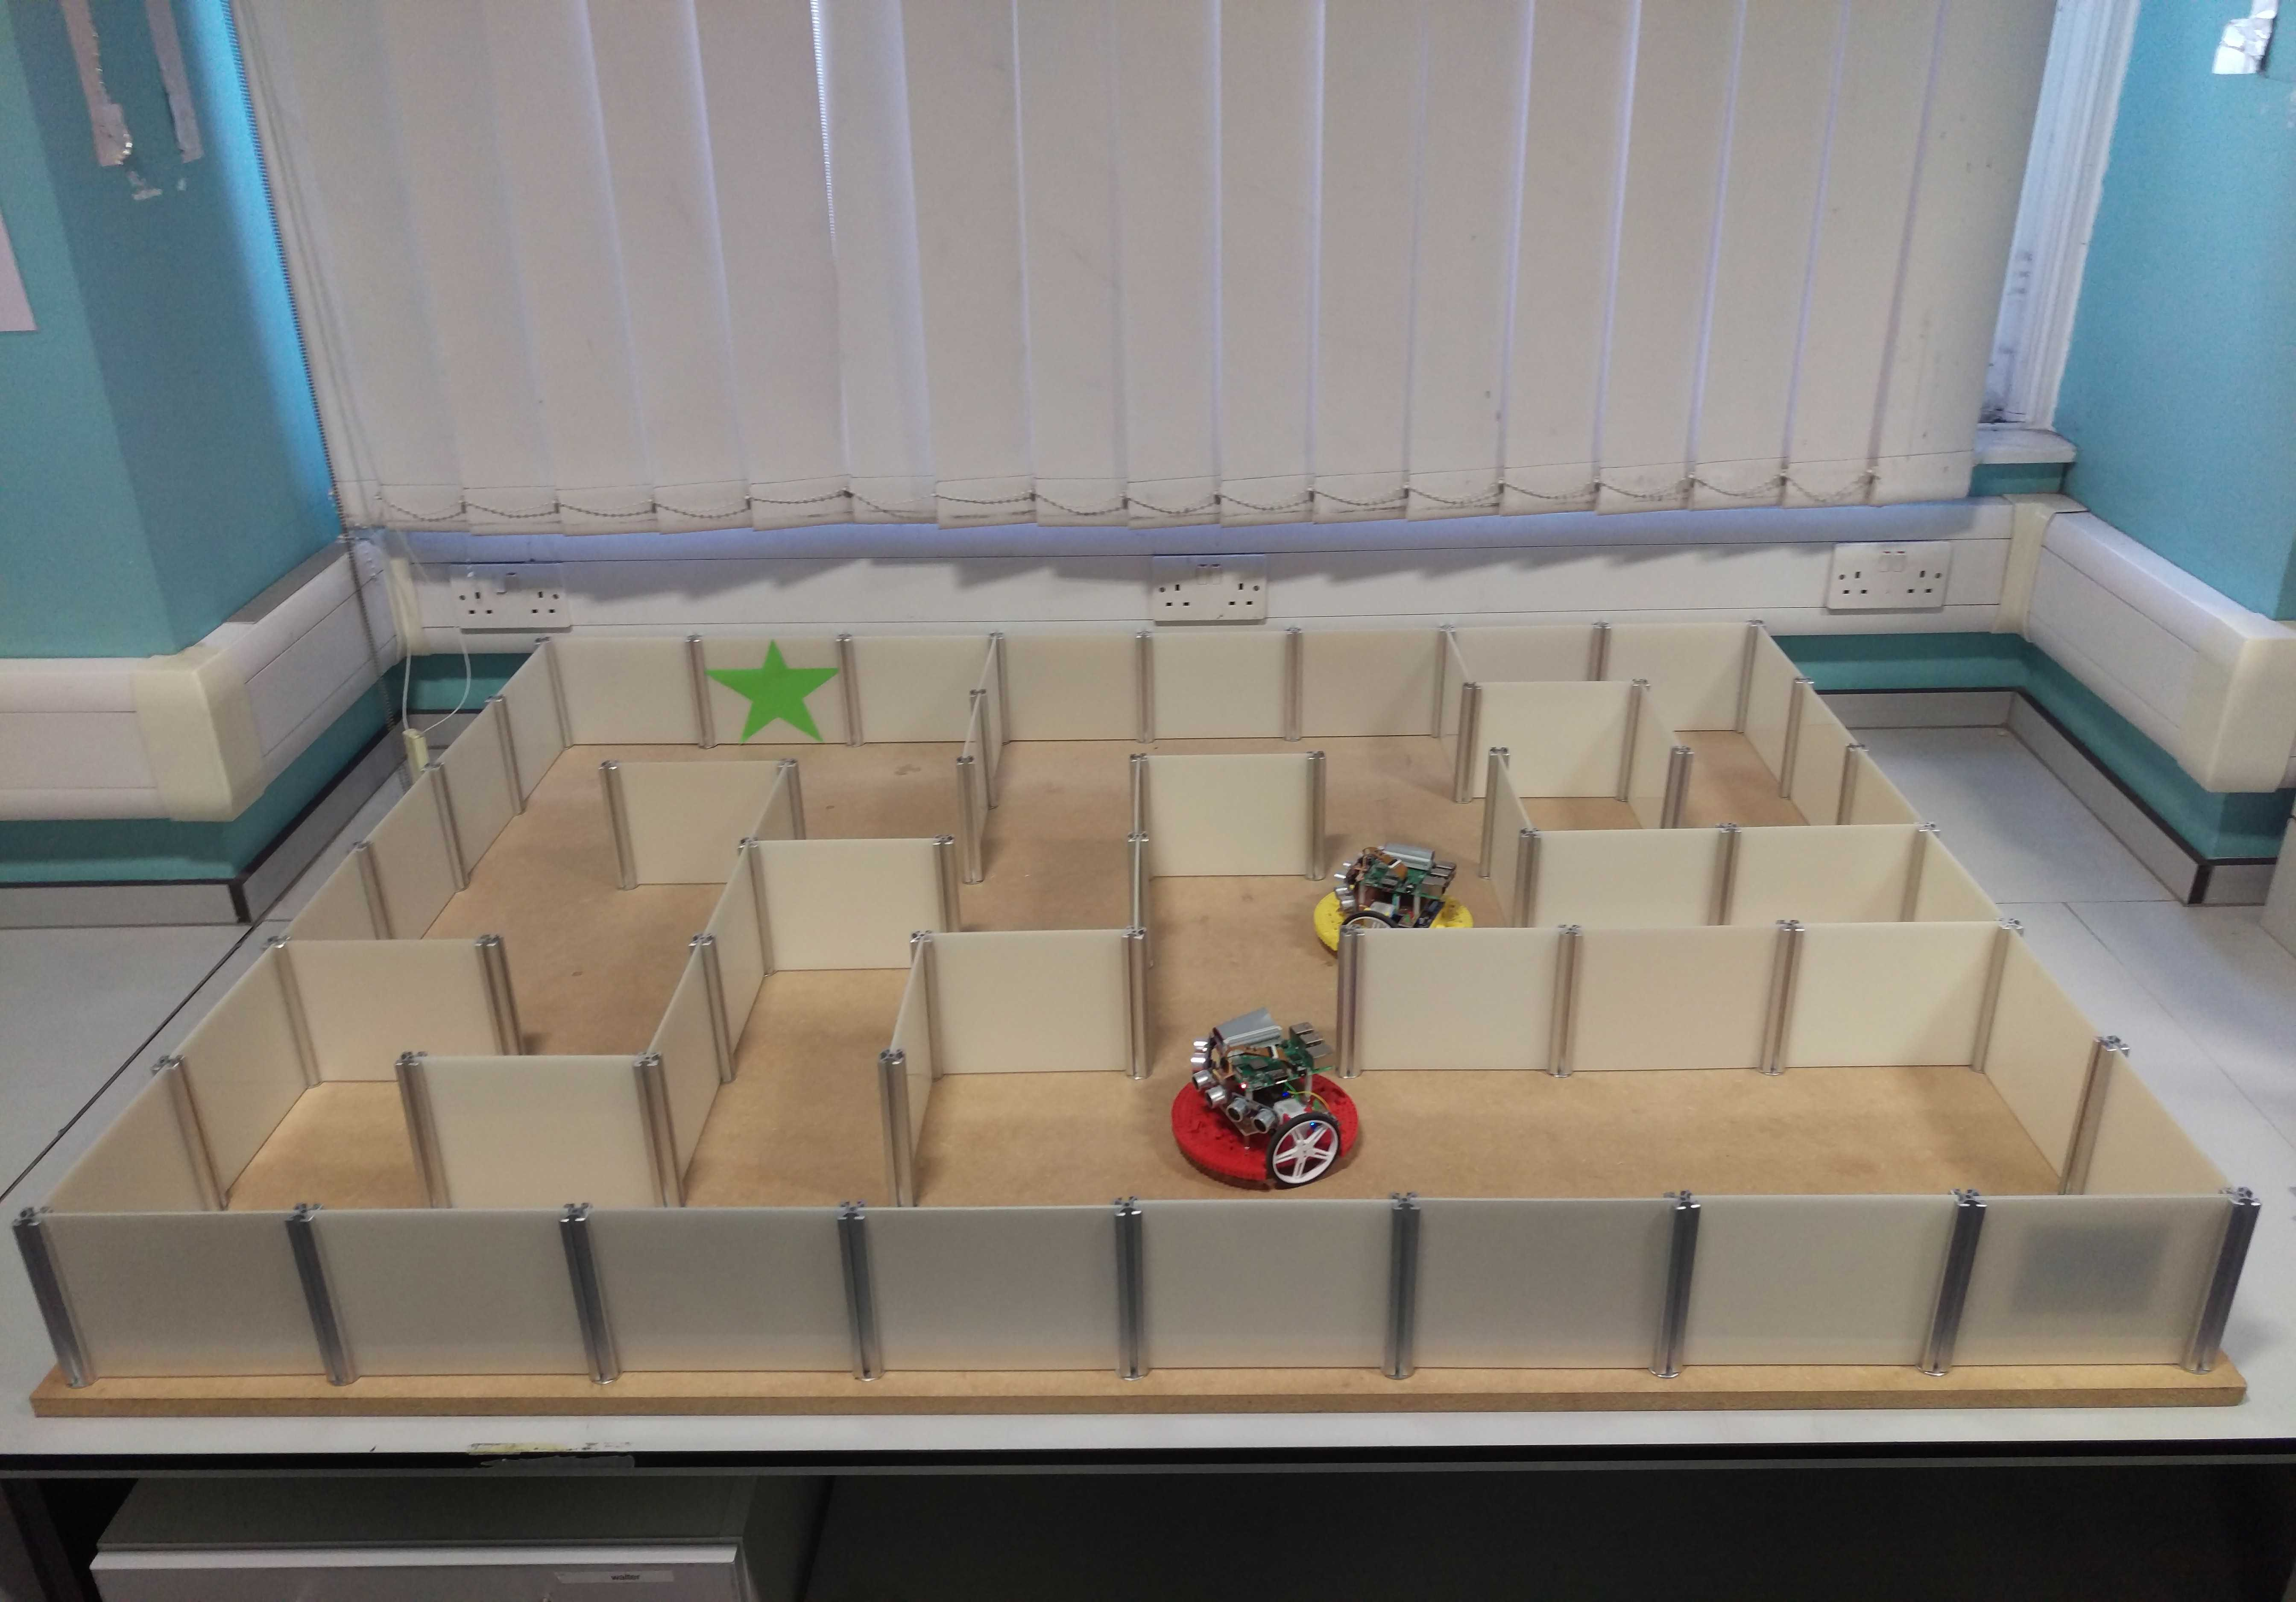
\includegraphics[width=0.8\textwidth]{diagrams/Maze4Real}
	\caption{An example maze configuration constructed using the maze}\label{fig:maze_pic}

\end{figure}


As can be seen from Table~\ref{maze_reqs_met}, the requirements laid out in the design
phase (see Section~\ref{test/maze/design}) were largely met with the only two
requirements not met being of medium or low priority.

\begin{table}[H]\centering
\caption{Modular maze requirements met
\label{maze_reqs_met}}
    \begin{tabular}{p{9cm}p{2cm}p{2cm}}
        \toprule
        \thead{Requirement} & \thead{Priority} & \thead{Met}\\
        \midrule
        Be easily modifiable & High & Met\\
        Have enough cells to allow varied mazes & High & Met\\
        Have minimum cell width $>$ diameter of the robot & High & Met\\
        Be accompanied by sufficient ``pegs'' and ``walls'' to build complex 		mazes & High & Met\\
        Wall material be non-translucent and non-reflective & Medium & Met\\
        Base material be non-reflective & Medium & Met\\
        Maze be easily transportable & Medium & Not Met\\
        Maze base be modular & Low & Not Met\\
        \bottomrule
    \end{tabular}
\end{table}
\section{Testing Strategy}\label{systest/strategy}
The testing strategy designed for system testing was to develop a number of
increasingly difficult mazes and test the capability of the robot to find a goal
in each of these mazes. Additional robots will then be added to each of these
configurations and the time recorded for quantitative testing of the project.

A number of maze configurations were drawn up to be used as the default test
cases for the robots. These configurations are shown in Figure~\ref{fig:maze_configs}. It is worth noting that these configurations were created before the
cell width of the maze was reduced and therefore, maze configurations with 1
cell width paths are significantly more difficult to traverse than previously
thought.

\begin{figure}[!ht]
  \centering
  \begin{subfigure}[b]{0.3\textwidth}
    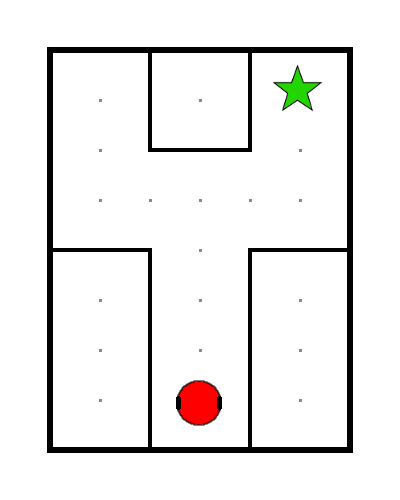
\includegraphics[width=\textwidth]{diagrams/maze_configuration_1}
    \caption{Configuration 1}
    \label{fig:maze_configs/1}
  \end{subfigure}
  ~
  \begin{subfigure}[b]{0.3\textwidth}
    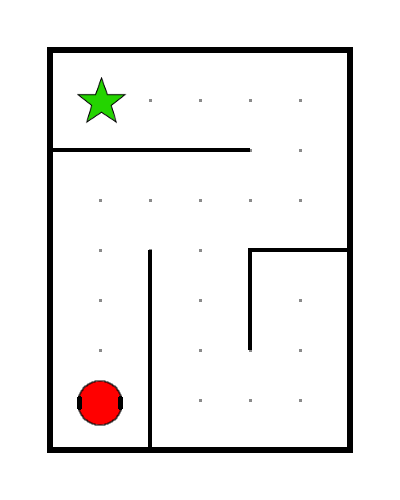
\includegraphics[width=\textwidth]{diagrams/maze_configuration_2}
    \caption{Configuration 2}
    \label{fig:maze_configs/2}
  \end{subfigure}

  \begin{subfigure}[b]{0.3\textwidth}
    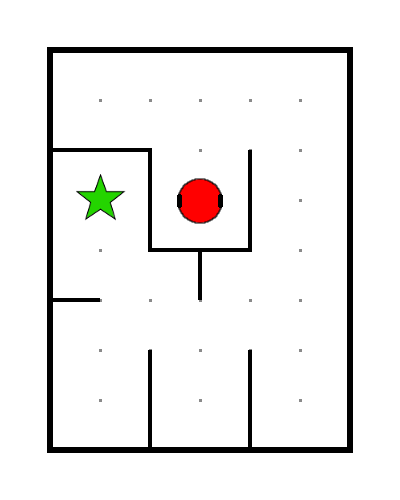
\includegraphics[width=\textwidth]{diagrams/maze_configuration_3}
    \caption{Configuration 3}
    \label{fig:maze_configs/3}
  \end{subfigure}
  ~
  \begin{subfigure}[b]{0.3\textwidth}
    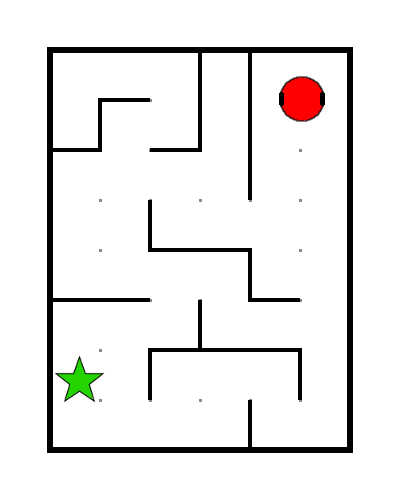
\includegraphics[width=\textwidth]{diagrams/maze_configuration_4}
    \caption{Configuration 4}
    \label{fig:maze_configs/4}
  \end{subfigure}
  \caption{Example maze configurations}\label{fig:maze_configs}
\end{figure}

\section{Results}\label{systest/results}
Due to the issues described with PID tuning and SLAM described in Sections~\ref{soft/PID} and ~\ref{soft/SLAM/tuning} respectively,
minimal system testing took place. The system tests which did take place were
without the SLAM/AI integration, so the AI had to make decisions without knowledge of the derived map. Despite this, the
system was tested on the maze configurations shown in Figure~\ref{fig:maze_configs} with one agent, and then again with two. These results are shown in Table~\ref{results}.

\begin{table}[!ht]\centering
\caption{Results
\label{results}}
    \begin{tabular}{cccccc}
        \toprule
        \thead{Maze \\configuration} & \thead{Avg. runtime with \\
        one agent [\si{\second}]} & \thead{Avg. runtime with \\
        two agents [\si{\second}]}\\
        \midrule
        1 & 57.8 & 22.7\\
        2 & 85.2 & 81.9\\
        3 & 80.6 & 71.2\\
        4 & 134.2 & 118.3\\
        \bottomrule
    \end{tabular}
\end{table}

The results shown are not indicative of the project had it been completed in its
entirety, however these results give benchmark scores for the shown maze
configurations using a very basic AI module. A major drawback of the lack of SLAM/AI
integration is that the same path can be searched multiple times, which resulted in a few
instances with unusually slow results. The results do broadly show, however,
that multiple agents perform better than a single agent in terms of speed of 
search. In these cases, this is a simple case of ``many hands make light
work'' rather than anything intelligent that the robots are doing.
Nevertheless, the results demonstrate the successful outcomes of the project
and vindicate the time taken to research the field of co-operative robotics.
Work detailed in further work (Section~\ref{furtherwork}) can use the
results shown here as benchmark results and
measure the success of refined SLAM and AI implementations against these results to
evaluate progress being made.
